\section{Introduction}
\label{sec:intro}

Wildlife management runs on counts. Deer density drives hunting quotas, culling decisions,
disease-response planning, and vehicle-collision mitigation, and those counts are still
produced largely by human observers riding transects at night with spotlights or handheld
thermal scopes. Automating the count is an obvious application of modern detection, and the
literature has largely treated it as one: train a detector on annotated animal imagery,
report mAP, and declare the survey problem addressed.

This paper argues, and then measures, that the two problems come apart. A detector is
rewarded for finding animals in \emph{frames}. A survey needs the number of distinct
\emph{animals}. Between those sits a chain of decisions --- associating detections into
tracks, deciding which tracks are real, deciding which are duplicates of an animal already
counted --- that no detection metric scores and that, we find, dominates the error.

\begin{figure}[t]
  \centering
  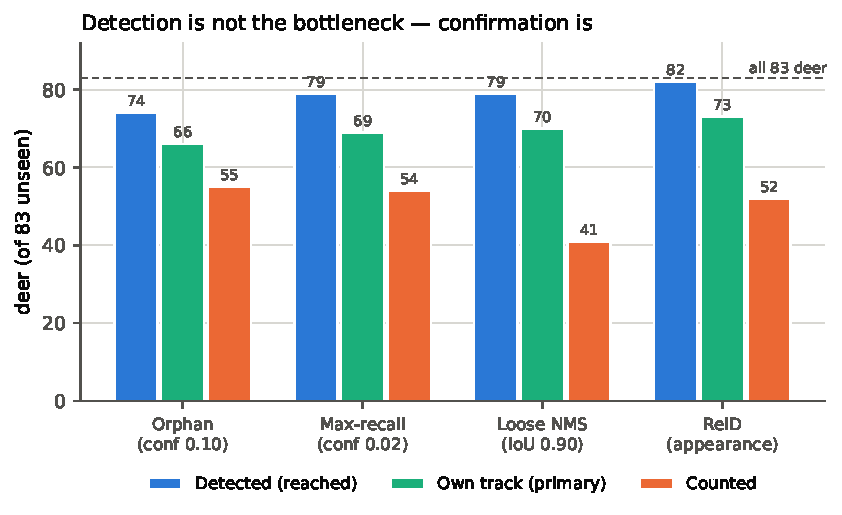
\includegraphics[width=\linewidth]{figures/fig1_funnel.pdf}
  \caption{\textbf{Detection is not the bottleneck.} Of the 83 deer in the 13 videos our
  detector never saw, up to 82 are found by \emph{some} candidate track and 73 acquire a
  distinct track of their own, but only 52--55 are counted. Every bar is one of four
  candidate-generation configurations (\cref{sec:counting}); improving the pool moves the
  blue and green bars up and the orange bar \emph{down}.}
  \label{fig:funnel}
\end{figure}

We study this on a corpus we built for the purpose: 32 FLIR thermal road transects from
four sites in Illinois, 521,930 frames at $640\times512$ and 60\,fps, with every individual
deer annotated as a distinct track --- 236 animals, 21,646 boxes. Because one annotated
track is one animal, the corpus supplies detection ground truth, tracking ground truth, and
count ground truth simultaneously, which is what makes the decomposition below possible.

Our central instrument is a three-stage decomposition of counting error. For each ground-truth
animal we ask whether it is \reachedq (touched by at least one candidate track), whether it
is \primaryq (some candidate covers it better than it covers any other animal, so a
one-count-per-track decision \emph{could} count it), and whether it is finally \countedq.
The gaps between these three numbers attribute error to detection, to association, and to
confirmation respectively. \Cref{fig:funnel} is the result, and it is the paper in one
picture: on unseen video the pipeline reaches 98.8\% of animals, gives 88.0\% their own
track, and counts 62.7\%.

Having localized the loss, we attack it. We improve candidate generation four independent
ways --- lowering detector confidence from 0.10 to 0.02, removing the tracker's
track-initialization gate, raising the NMS IoU threshold from 0.50 to 0.90, and adding
appearance re-identification to the association step. Each one demonstrably improves the
pool. Each one makes the final count worse or no better. We then replace the hand-tuned
confirmation rule with learned alternatives of varying capacity, under three evaluation
protocols, and every one of them loses to three hand-tuned parameters.

That pair of negative results is not a failure to find a method; it is the finding. The
confirmation stage is starved not of capacity but of supervision: roughly 200 positive
tracks against 7{,}000--28{,}000 negatives, with the positives not linearly separable from
the duplicates in any feature we measured. Growing the candidate pool grows the negatives
far faster than the positives, which is exactly why every pool improvement hurts.

\paragraph{Contributions.}
\begin{enumerate}\itemsep2pt \parskip0pt \parsep0pt
\item \textbf{A thermal wildlife counting benchmark.} 32 fully annotated road-transect
videos, 521,930 frames, 236 individually tracked deer, with per-individual identity that
makes detection, tracking, and counting evaluable on one corpus. Released with the
evaluation harness.
\item \textbf{A decomposition that localizes counting error} into detection, association,
and confirmation (\reachedq/\primaryq/\countedq), and a held-out protocol that prevents the
optimism we found in the naive evaluation --- reporting counting accuracy on videos the
detector trained on inflates it by 33 points.
\item \textbf{Evidence that improving candidate generation degrades counting}, replicated
across four independent interventions, and evidence across three protocols that learned
confirmation does not beat a three-parameter rule at this data scale.
\item \textbf{A measurement finding with consequences beyond this dataset:} the
IoU$\geq$0.50 criterion re-ranks detectors relative to a counting-appropriate criterion, so
selecting a detector by its detection metric does not select the model that counts best.
\item \textbf{A quantified resolution limit for individual re-identification} at this pixel
scale, and the diagnosis of a training-distribution hole that makes the detector fail on
\emph{large} animals.
\end{enumerate}
